\section{ROOMLanguage}
	Real Time Object Oriented Modeling (ROOM) is a language ... 
	
		\subsection{LogicalModel}
		The LogicalModel describes the logical structure and behavior of a ROOM application. The LogicalModel an its elements can be mapped on any PhysicalModel and its elements...
	
		
		
		\subsubsection{ActorClass}
			\hypertarget{ref:ActorClass}{}
			
			The actor is the basic structural building block for building systems with ROOM. An actor can be refined hierarchically and thus can be of arbitrarily large scope. Ports define the interface of an actor. An actor can also have a behavior usually defined by a finite state machine. 
			
			
			\vspace{\baselineskip}
			\begingroup
			%\setlength{\tabcolsep}{10pt} % Default value: 6pt
			\renewcommand{\arraystretch}{1.8} % Default value: 1
			\parbox{\textwidth}{
			\begin{longtable}{l l p{.7\textwidth}}
				\multicolumn{2}{l}{\textbf{\large Features}} & \\
				\hline
			\multirow{9}{*}{Contains:} & \tabitem \hyperlink{ref:ActorRef}{ActorRef}  & An ActorRef ...description\\
			& \tabitem \hyperlink{ref:Port}{Port}  & A Port is an instance of a ProtocolClass and the only interface for an ActorClass. It provides strong decoupling of ActorClasses from each other, thus enabling easy testability, reusability and deployment of Actors to different threads or nodes.description  \\
			& \tabitem \hyperlink{ref:SAP}{SAP}  & An SAP ....description  \\
			& \tabitem \hyperlink{ref:SPP}{SPP}  & An SPP ... description \\
			& \tabitem \hyperlink{ref:Binding}{Binding}  & A Binding connects two Ports with each otherdescription \\
			& \tabitem \hyperlink{ref:LayerConnection}{LayerConnection}  & A LayerConnection ... description  \\
			& \tabitem \hyperlink{ref:Attribute}{Attribute}  & An Attribute is a member variable of a class (ActorClass, ProtocolClass, DataClass, ...)description  \\
			& \tabitem \hyperlink{ref:Operation}{Operation}  & An Operation is a member function of a class (ActorClass, ProtocolClass, DataClass, ...)description  \\
			& \tabitem \hyperlink{ref:StateMachine}{StateMachine}  & A StateMachine describes the state based, event driven behavior of an ActorClass \\
			\hline
			Uses: & \tabitem \hyperlink{ref:Inheritance}{Inheritance}  & Inheritance bla\\
			\hline
			\end{longtable}	
			}
			\endgroup
			\vspace{\baselineskip}
			
			\vspace{\baselineskip}
			\begingroup
			%\setlength{\tabcolsep}{10pt} % Default value: 6pt
			\renewcommand{\arraystretch}{1.8} % Default value: 1
			\parbox{\textwidth}{
			\begin{longtable}{l l p{.6\textwidth}}
				\multicolumn{2}{l}{\textbf{\large Related Features}} & \\
				\hline
			Typecasts: & \tabitem \hyperlink{ref:ActorRef}{ActorRef}  & An ActorRef ...description\\
			\hline
			Is contained in: & \tabitem \hyperlink{ref:LogicalModel}{LogicalModel}  & The LogicalModel describes the logical structure and behavior of a ROOM application. The LogicalModel an its elements can be mapped on any PhysicalModel and its elements...\\
			\hline
			Is edited by: & \tabitem \hyperlink{ref:GraphicalStructureEditor}{GraphicalStructureEditor}  & The Structure Editor allows to edit the Actor Structure in a convenient way. It is possible to create and arrange actor references and ports and to create bindings and layer connections.\\
			\hline
			\end{longtable}	
			}
			\endgroup
			\vspace{\baselineskip}
			
			some more about ActorClass, graphical and textual notation, concepts, ...
			
			\textbf{Example}
			\\
			\textbf{Graphical Notation}
			\\
				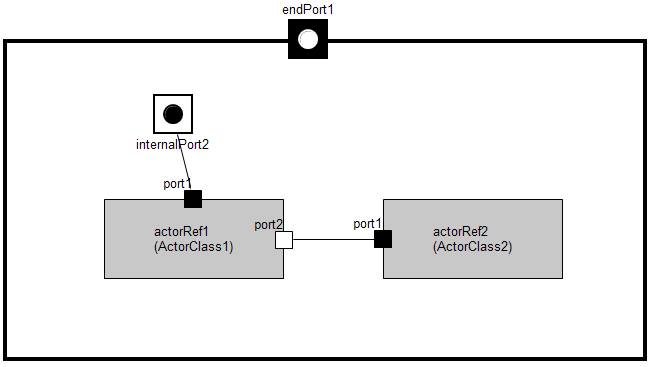
\includegraphics[width=\textwidth]{images/300-SimpleActorClassStructure.png}
			\\
			\textbf{Textual Notation}
			\\
				\begin{lstlisting}[language=ROOM]
				ActorClass SimpleActorClass {
					Interface {
						Port endPort1: PSimpleProtocolClass
					}
					Structure {
						external Port endPort1
						conjugated Port internalPort2: PSimpleProtocolClass
			
						ActorRef actorRef1: ActorClass1
						ActorRef actorRef2: ActorClass2
						Binding actorRef1.port2 and actorRef2.port1
						Binding internalPort2 and actorRef1.port1
					}
					Behavior {
						StateMachine {
							Transition init: initial -> State1
							State State1
						}
					}
				}
				\end{lstlisting}
		
		\subsubsection{ActorRef}
			\hypertarget{ref:ActorRef}{}
			
			An ActorRef ...description
			
			\vspace{\baselineskip}
			\begingroup
			%\setlength{\tabcolsep}{10pt} % Default value: 6pt
			\renewcommand{\arraystretch}{1.8} % Default value: 1
			\parbox{\textwidth}{
			\begin{longtable}{l p{.8\textwidth}}
				\multicolumn{2}{l}{\textbf{\large Properties}} \\
				\hline
			\tabitem multiplicity & \\
			\end{longtable}	
			}
			\endgroup
			\vspace{\baselineskip}
			
			\vspace{\baselineskip}
			\begingroup
			%\setlength{\tabcolsep}{10pt} % Default value: 6pt
			\renewcommand{\arraystretch}{1.8} % Default value: 1
			\parbox{\textwidth}{
			\begin{longtable}{l l p{.7\textwidth}}
				\multicolumn{2}{l}{\textbf{\large Features}} & \\
				\hline
			Is of type: & \tabitem \hyperlink{ref:ActorClass}{ActorClass}  & The actor is the basic structural building block for building systems with ROOM. An actor can be refined hierarchically and thus can be of arbitrarily large scope. Ports define the interface of an actor. An actor can also have a behavior usually defined by a finite state machine. \\
			\hline
			\end{longtable}	
			}
			\endgroup
			\vspace{\baselineskip}
			
			\vspace{\baselineskip}
			\begingroup
			%\setlength{\tabcolsep}{10pt} % Default value: 6pt
			\renewcommand{\arraystretch}{1.8} % Default value: 1
			\parbox{\textwidth}{
			\begin{longtable}{l l p{.6\textwidth}}
				\multicolumn{2}{l}{\textbf{\large Related Features}} & \\
				\hline
			\multirow{2}{*}{Is contained in:} & \tabitem \hyperlink{ref:ActorClass}{ActorClass}  & The actor is the basic structural building block for building systems with ROOM. An actor can be refined hierarchically and thus can be of arbitrarily large scope. Ports define the interface of an actor. An actor can also have a behavior usually defined by a finite state machine. \\
			& \tabitem \hyperlink{ref:SubSystemClass}{SubSystemClass}  & The SubSystem is main Actor of an executable part of the system. It instantiates the Actor instance tree instance of the application ...
				
				Actor instance tree example:
			 \\
			\hline
			\multirow{2}{*}{Is edited by:} & \tabitem \hyperlink{ref:ActorRefPropertyDialog}{ActorRefPropertyDialog}  & A Dialog to edit structural reference of an ActorRef.
			\\
			& \tabitem \hyperlink{ref:GraphicalStructureEditor}{GraphicalStructureEditor}  & The Structure Editor allows to edit the Actor Structure in a convenient way. It is possible to create and arrange actor references and ports and to create bindings and layer connections. \\
			\hline
			\end{longtable}	
			}
			\endgroup
			\vspace{\baselineskip}
			
			
		
		\subsubsection{Attribute}
			\hypertarget{ref:Attribute}{}
			
			An Attribute is a member variable of a class (ActorClass, ProtocolClass, DataClass, ...)description 
			
			\vspace{\baselineskip}
			\begingroup
			%\setlength{\tabcolsep}{10pt} % Default value: 6pt
			\renewcommand{\arraystretch}{1.8} % Default value: 1
			\parbox{\textwidth}{
			\begin{longtable}{l p{.8\textwidth}}
				\multicolumn{2}{l}{\textbf{\large Properties}} \\
				\hline
			\tabitem defaultValueLiteral & \\
			\tabitem size & \\
			\end{longtable}	
			}
			\endgroup
			\vspace{\baselineskip}
			
			\vspace{\baselineskip}
			\begingroup
			%\setlength{\tabcolsep}{10pt} % Default value: 6pt
			\renewcommand{\arraystretch}{1.8} % Default value: 1
			\parbox{\textwidth}{
			\begin{longtable}{l l p{.7\textwidth}}
				\multicolumn{2}{l}{\textbf{\large Features}} & \\
				\hline
			Is of type: & \tabitem \hyperlink{ref:DataType}{DataType}  & is abstractdescription\\
			\hline
			\end{longtable}	
			}
			\endgroup
			\vspace{\baselineskip}
			
			\vspace{\baselineskip}
			\begingroup
			%\setlength{\tabcolsep}{10pt} % Default value: 6pt
			\renewcommand{\arraystretch}{1.8} % Default value: 1
			\parbox{\textwidth}{
			\begin{longtable}{l l p{.6\textwidth}}
				\multicolumn{2}{l}{\textbf{\large Related Features}} & \\
				\hline
			\multirow{3}{*}{Is contained in:} & \tabitem \hyperlink{ref:ActorClass}{ActorClass}  & The actor is the basic structural building block for building systems with ROOM. An actor can be refined hierarchically and thus can be of arbitrarily large scope. Ports define the interface of an actor. An actor can also have a behavior usually defined by a finite state machine. \\
			& \tabitem \hyperlink{ref:DataClass}{DataClass}  & A DataClass ...description  \\
			& \tabitem \hyperlink{ref:ProtocolClass}{ProtocolClass}  & A ProtocolClass contains the Interface specification for a Port. It can provide one of three different CommunicationTypes (eventdriven, datadriven, sync).description  \\
			\hline
			\end{longtable}	
			}
			\endgroup
			\vspace{\baselineskip}
			
			
		
		\subsubsection{Binding}
			\hypertarget{ref:Binding}{}
			
			A Binding connects two Ports with each otherdescription
			
			
			\vspace{\baselineskip}
			\begingroup
			%\setlength{\tabcolsep}{10pt} % Default value: 6pt
			\renewcommand{\arraystretch}{1.8} % Default value: 1
			\parbox{\textwidth}{
			\begin{longtable}{l l p{.7\textwidth}}
				\multicolumn{2}{l}{\textbf{\large Features}} & \\
				\hline
			\multirow{2}{*}{Uses:} & \tabitem \hyperlink{ref:Port}{Port} : endpoint1 & A Port is an instance of a ProtocolClass and the only interface for an ActorClass. It provides strong decoupling of ActorClasses from each other, thus enabling easy testability, reusability and deployment of Actors to different threads or nodes.description \\
			& \tabitem \hyperlink{ref:Port}{Port} : endpoint2 & A Port is an instance of a ProtocolClass and the only interface for an ActorClass. It provides strong decoupling of ActorClasses from each other, thus enabling easy testability, reusability and deployment of Actors to different threads or nodes.description  \\
			\hline
			\end{longtable}	
			}
			\endgroup
			\vspace{\baselineskip}
			
			\vspace{\baselineskip}
			\begingroup
			%\setlength{\tabcolsep}{10pt} % Default value: 6pt
			\renewcommand{\arraystretch}{1.8} % Default value: 1
			\parbox{\textwidth}{
			\begin{longtable}{l l p{.6\textwidth}}
				\multicolumn{2}{l}{\textbf{\large Related Features}} & \\
				\hline
			\multirow{3}{*}{Is contained in:} & \tabitem \hyperlink{ref:ActorClass}{ActorClass}  & The actor is the basic structural building block for building systems with ROOM. An actor can be refined hierarchically and thus can be of arbitrarily large scope. Ports define the interface of an actor. An actor can also have a behavior usually defined by a finite state machine. \\
			& \tabitem \hyperlink{ref:LogicalSystem}{LogicalSystem}  &  \\
			& \tabitem \hyperlink{ref:SubSystemClass}{SubSystemClass}  & The SubSystem is main Actor of an executable part of the system. It instantiates the Actor instance tree instance of the application ...
				
				Actor instance tree example:
			 \\
			\hline
			Is edited by: & \tabitem \hyperlink{ref:GraphicalStructureEditor}{GraphicalStructureEditor}  & The Structure Editor allows to edit the Actor Structure in a convenient way. It is possible to create and arrange actor references and ports and to create bindings and layer connections.\\
			\hline
			\end{longtable}	
			}
			\endgroup
			\vspace{\baselineskip}
			
			
		
		\subsubsection{CommunicationType}
			\hypertarget{ref:CommunicationType}{}
			
			CommunicationTypedescription
			
			
			
			\vspace{\baselineskip}
			\begingroup
			%\setlength{\tabcolsep}{10pt} % Default value: 6pt
			\renewcommand{\arraystretch}{1.8} % Default value: 1
			\parbox{\textwidth}{
			\begin{longtable}{l l p{.6\textwidth}}
				\multicolumn{2}{l}{\textbf{\large Related Features}} & \\
				\hline
			\multirow{3}{*}{Inheriting features:} & \tabitem \hyperlink{ref:datadrivenCommunicationType}{datadrivenCommunicationType}  & datadriven bla...description\\
			& \tabitem \hyperlink{ref:eventdrivenCommunicationType}{eventdrivenCommunicationType}  & eventdriven bla...description \\
			& \tabitem \hyperlink{ref:syncCommunicationType}{syncCommunicationType}  & CommunicationType sync bla...description  \\
			\hline
			Is contained in: & \tabitem \hyperlink{ref:ProtocolClass}{ProtocolClass}  & A ProtocolClass contains the Interface specification for a Port. It can provide one of three different CommunicationTypes (eventdriven, datadriven, sync).description \\
			\hline
			\end{longtable}	
			}
			\endgroup
			\vspace{\baselineskip}
			
			
		
		\subsubsection{DataType}
			\hypertarget{ref:DataType}{}
			
			is abstractdescription
			
			
			
			\vspace{\baselineskip}
			\begingroup
			%\setlength{\tabcolsep}{10pt} % Default value: 6pt
			\renewcommand{\arraystretch}{1.8} % Default value: 1
			\parbox{\textwidth}{
			\begin{longtable}{l l p{.6\textwidth}}
				\multicolumn{2}{l}{\textbf{\large Related Features}} & \\
				\hline
			\multirow{4}{*}{Inheriting features:} & \tabitem \hyperlink{ref:DataClass}{DataClass}  & A DataClass ...description \\
			& \tabitem \hyperlink{ref:EnumerationType}{EnumerationType}  & An EnumerationType ...description  \\
			& \tabitem \hyperlink{ref:ExternalType}{ExternalType}  & An ExternalType ...description  \\
			& \tabitem \hyperlink{ref:PrimitiveType}{PrimitiveType}  & A PrimitiveType ...description \\
			\hline
			Typecasts: & \tabitem \hyperlink{ref:Attribute}{Attribute}  & An Attribute is a member variable of a class (ActorClass, ProtocolClass, DataClass, ...)description \\
			\hline
			Is contained in: & \tabitem \hyperlink{ref:LogicalModel}{LogicalModel}  & The LogicalModel describes the logical structure and behavior of a ROOM application. The LogicalModel an its elements can be mapped on any PhysicalModel and its elements...\\
			\hline
			\end{longtable}	
			}
			\endgroup
			\vspace{\baselineskip}
			
			
		
		\subsubsection{LayerConnection}
			\hypertarget{ref:LayerConnection}{}
			
			A LayerConnection ... description 
			
			
			\vspace{\baselineskip}
			\begingroup
			%\setlength{\tabcolsep}{10pt} % Default value: 6pt
			\renewcommand{\arraystretch}{1.8} % Default value: 1
			\parbox{\textwidth}{
			\begin{longtable}{l l p{.7\textwidth}}
				\multicolumn{2}{l}{\textbf{\large Features}} & \\
				\hline
			\multirow{2}{*}{Uses:} & \tabitem \hyperlink{ref:SAP}{SAP} : saPoint & An SAP ....description \\
			& \tabitem \hyperlink{ref:SPP}{SPP} : spPoint & An SPP ... description \\
			\hline
			\end{longtable}	
			}
			\endgroup
			\vspace{\baselineskip}
			
			\vspace{\baselineskip}
			\begingroup
			%\setlength{\tabcolsep}{10pt} % Default value: 6pt
			\renewcommand{\arraystretch}{1.8} % Default value: 1
			\parbox{\textwidth}{
			\begin{longtable}{l l p{.6\textwidth}}
				\multicolumn{2}{l}{\textbf{\large Related Features}} & \\
				\hline
			\multirow{3}{*}{Is contained in:} & \tabitem \hyperlink{ref:ActorClass}{ActorClass}  & The actor is the basic structural building block for building systems with ROOM. An actor can be refined hierarchically and thus can be of arbitrarily large scope. Ports define the interface of an actor. An actor can also have a behavior usually defined by a finite state machine. \\
			& \tabitem \hyperlink{ref:LogicalSystem}{LogicalSystem}  &  \\
			& \tabitem \hyperlink{ref:SubSystemClass}{SubSystemClass}  & The SubSystem is main Actor of an executable part of the system. It instantiates the Actor instance tree instance of the application ...
				
				Actor instance tree example:
			 \\
			\hline
			Is edited by: & \tabitem \hyperlink{ref:GraphicalStructureEditor}{GraphicalStructureEditor}  & The Structure Editor allows to edit the Actor Structure in a convenient way. It is possible to create and arrange actor references and ports and to create bindings and layer connections.\\
			\hline
			\end{longtable}	
			}
			\endgroup
			\vspace{\baselineskip}
			
			
		
		\subsubsection{Operation}
			\hypertarget{ref:Operation}{}
			
			An Operation is a member function of a class (ActorClass, ProtocolClass, DataClass, ...)description 
			
			\vspace{\baselineskip}
			\begingroup
			%\setlength{\tabcolsep}{10pt} % Default value: 6pt
			\renewcommand{\arraystretch}{1.8} % Default value: 1
			\parbox{\textwidth}{
			\begin{longtable}{l p{.8\textwidth}}
				\multicolumn{2}{l}{\textbf{\large Properties}} \\
				\hline
			\tabitem returnType & \\
			\tabitem arguments & \\
			\end{longtable}	
			}
			\endgroup
			\vspace{\baselineskip}
			
			
			\vspace{\baselineskip}
			\begingroup
			%\setlength{\tabcolsep}{10pt} % Default value: 6pt
			\renewcommand{\arraystretch}{1.8} % Default value: 1
			\parbox{\textwidth}{
			\begin{longtable}{l l p{.6\textwidth}}
				\multicolumn{2}{l}{\textbf{\large Related Features}} & \\
				\hline
			\multirow{3}{*}{Is contained in:} & \tabitem \hyperlink{ref:ActorClass}{ActorClass}  & The actor is the basic structural building block for building systems with ROOM. An actor can be refined hierarchically and thus can be of arbitrarily large scope. Ports define the interface of an actor. An actor can also have a behavior usually defined by a finite state machine. \\
			& \tabitem \hyperlink{ref:DataClass}{DataClass}  & A DataClass ...description  \\
			& \tabitem \hyperlink{ref:ProtocolClass}{ProtocolClass}  & A ProtocolClass contains the Interface specification for a Port. It can provide one of three different CommunicationTypes (eventdriven, datadriven, sync).description  \\
			\hline
			\end{longtable}	
			}
			\endgroup
			\vspace{\baselineskip}
			
			
		
		\subsubsection{Port}
			\hypertarget{ref:Port}{}
			
			A Port is an instance of a ProtocolClass and the only interface for an ActorClass. It provides strong decoupling of ActorClasses from each other, thus enabling easy testability, reusability and deployment of Actors to different threads or nodes.description 
			
			\vspace{\baselineskip}
			\begingroup
			%\setlength{\tabcolsep}{10pt} % Default value: 6pt
			\renewcommand{\arraystretch}{1.8} % Default value: 1
			\parbox{\textwidth}{
			\begin{longtable}{l p{.8\textwidth}}
				\multicolumn{2}{l}{\textbf{\large Properties}} \\
				\hline
			\tabitem conjugated & \\
			\tabitem multiplicity & \\
			\end{longtable}	
			}
			\endgroup
			\vspace{\baselineskip}
			
			\vspace{\baselineskip}
			\begingroup
			%\setlength{\tabcolsep}{10pt} % Default value: 6pt
			\renewcommand{\arraystretch}{1.8} % Default value: 1
			\parbox{\textwidth}{
			\begin{longtable}{l l p{.7\textwidth}}
				\multicolumn{2}{l}{\textbf{\large Features}} & \\
				\hline
			Is of type: & \tabitem \hyperlink{ref:ProtocolClass}{ProtocolClass}  & A ProtocolClass contains the Interface specification for a Port. It can provide one of three different CommunicationTypes (eventdriven, datadriven, sync).description \\
			\hline
			\end{longtable}	
			}
			\endgroup
			\vspace{\baselineskip}
			
			\vspace{\baselineskip}
			\begingroup
			%\setlength{\tabcolsep}{10pt} % Default value: 6pt
			\renewcommand{\arraystretch}{1.8} % Default value: 1
			\parbox{\textwidth}{
			\begin{longtable}{l l p{.6\textwidth}}
				\multicolumn{2}{l}{\textbf{\large Related Features}} & \\
				\hline
			\multirow{3}{*}{Inheriting features:} & \tabitem \hyperlink{ref:ExternalEndPort}{ExternalEndPort}  & ExternalEndPort description\\
			& \tabitem \hyperlink{ref:InternalEndPort}{InternalEndPort}  & InternalEndPort description \\
			& \tabitem \hyperlink{ref:RelayPort}{RelayPort}  & RelayPort description \\
			\hline
			Is contained in: & \tabitem \hyperlink{ref:ActorClass}{ActorClass}  & The actor is the basic structural building block for building systems with ROOM. An actor can be refined hierarchically and thus can be of arbitrarily large scope. Ports define the interface of an actor. An actor can also have a behavior usually defined by a finite state machine. \\
			\hline
			\multirow{2}{*}{Is edited by:} & \tabitem \hyperlink{ref:GraphicalStructureEditor}{GraphicalStructureEditor}  & The Structure Editor allows to edit the Actor Structure in a convenient way. It is possible to create and arrange actor references and ports and to create bindings and layer connections.\\
			& \tabitem \hyperlink{ref:PortPropertyDialog}{PortPropertyDialog}  &  \\
			\hline
			\multirow{2}{*}{Is used by:} & \tabitem \hyperlink{ref:Binding}{Binding} : endpoint1 & A Binding connects two Ports with each otherdescription\\
			& \tabitem \hyperlink{ref:Binding}{Binding} : endpoint2 & A Binding connects two Ports with each otherdescription \\
			\hline
			\end{longtable}	
			}
			\endgroup
			\vspace{\baselineskip}
			
			
		
		\subsubsection{ProtocolClass}
			\hypertarget{ref:ProtocolClass}{}
			
			A ProtocolClass contains the Interface specification for a Port. It can provide one of three different CommunicationTypes (eventdriven, datadriven, sync).description 
			
			
			\vspace{\baselineskip}
			\begingroup
			%\setlength{\tabcolsep}{10pt} % Default value: 6pt
			\renewcommand{\arraystretch}{1.8} % Default value: 1
			\parbox{\textwidth}{
			\begin{longtable}{l l p{.7\textwidth}}
				\multicolumn{2}{l}{\textbf{\large Features}} & \\
				\hline
			\multirow{3}{*}{Contains:} & \tabitem \hyperlink{ref:Attribute}{Attribute}  & An Attribute is a member variable of a class (ActorClass, ProtocolClass, DataClass, ...)description \\
			& \tabitem \hyperlink{ref:Operation}{Operation}  & An Operation is a member function of a class (ActorClass, ProtocolClass, DataClass, ...)description  \\
			& \tabitem \hyperlink{ref:CommunicationType}{CommunicationType}  & CommunicationTypedescription \\
			\hline
			Uses: & \tabitem \hyperlink{ref:Inheritance}{Inheritance}  & Inheritance bla\\
			\hline
			\end{longtable}	
			}
			\endgroup
			\vspace{\baselineskip}
			
			\vspace{\baselineskip}
			\begingroup
			%\setlength{\tabcolsep}{10pt} % Default value: 6pt
			\renewcommand{\arraystretch}{1.8} % Default value: 1
			\parbox{\textwidth}{
			\begin{longtable}{l l p{.6\textwidth}}
				\multicolumn{2}{l}{\textbf{\large Related Features}} & \\
				\hline
			\multirow{3}{*}{Typecasts:} & \tabitem \hyperlink{ref:Port}{Port}  & A Port is an instance of a ProtocolClass and the only interface for an ActorClass. It provides strong decoupling of ActorClasses from each other, thus enabling easy testability, reusability and deployment of Actors to different threads or nodes.description \\
			& \tabitem \hyperlink{ref:SAP}{SAP}  & An SAP ....description  \\
			& \tabitem \hyperlink{ref:SPP}{SPP}  & An SPP ... description \\
			\hline
			Is contained in: & \tabitem \hyperlink{ref:LogicalModel}{LogicalModel}  & The LogicalModel describes the logical structure and behavior of a ROOM application. The LogicalModel an its elements can be mapped on any PhysicalModel and its elements...\\
			\hline
			\end{longtable}	
			}
			\endgroup
			\vspace{\baselineskip}
			
			
		
		\subsubsection{RelayPort}
			\hypertarget{ref:RelayPort}{}
			
			RelayPort description
			
			
			\vspace{\baselineskip}
			\begingroup
			%\setlength{\tabcolsep}{10pt} % Default value: 6pt
			\renewcommand{\arraystretch}{1.8} % Default value: 1
			\parbox{\textwidth}{
			\begin{longtable}{l l p{.7\textwidth}}
				\multicolumn{2}{l}{\textbf{\large Features}} & \\
				\hline
			Is a: & \tabitem \hyperlink{ref:Port}{Port}  & A Port is an instance of a ProtocolClass and the only interface for an ActorClass. It provides strong decoupling of ActorClasses from each other, thus enabling easy testability, reusability and deployment of Actors to different threads or nodes.description \\
			\hline
			\end{longtable}	
			}
			\endgroup
			\vspace{\baselineskip}
			
			\vspace{\baselineskip}
			\begingroup
			%\setlength{\tabcolsep}{10pt} % Default value: 6pt
			\renewcommand{\arraystretch}{1.8} % Default value: 1
			\parbox{\textwidth}{
			\begin{longtable}{l l p{.6\textwidth}}
				\multicolumn{2}{l}{\textbf{\large Related Features}} & \\
				\hline
			Is contained in: & \tabitem \hyperlink{ref:SubSystemClass}{SubSystemClass}  & The SubSystem is main Actor of an executable part of the system. It instantiates the Actor instance tree instance of the application ...
				
				Actor instance tree example:
			\\
			\hline
			\end{longtable}	
			}
			\endgroup
			\vspace{\baselineskip}
			
			
		
		\subsubsection{SAP}
			\hypertarget{ref:SAP}{}
			
			An SAP ....description 
			
			
			\vspace{\baselineskip}
			\begingroup
			%\setlength{\tabcolsep}{10pt} % Default value: 6pt
			\renewcommand{\arraystretch}{1.8} % Default value: 1
			\parbox{\textwidth}{
			\begin{longtable}{l l p{.7\textwidth}}
				\multicolumn{2}{l}{\textbf{\large Features}} & \\
				\hline
			Is of type: & \tabitem \hyperlink{ref:ProtocolClass}{ProtocolClass}  & A ProtocolClass contains the Interface specification for a Port. It can provide one of three different CommunicationTypes (eventdriven, datadriven, sync).description \\
			\hline
			\end{longtable}	
			}
			\endgroup
			\vspace{\baselineskip}
			
			\vspace{\baselineskip}
			\begingroup
			%\setlength{\tabcolsep}{10pt} % Default value: 6pt
			\renewcommand{\arraystretch}{1.8} % Default value: 1
			\parbox{\textwidth}{
			\begin{longtable}{l l p{.6\textwidth}}
				\multicolumn{2}{l}{\textbf{\large Related Features}} & \\
				\hline
			Is contained in: & \tabitem \hyperlink{ref:ActorClass}{ActorClass}  & The actor is the basic structural building block for building systems with ROOM. An actor can be refined hierarchically and thus can be of arbitrarily large scope. Ports define the interface of an actor. An actor can also have a behavior usually defined by a finite state machine. \\
			\hline
			Is edited by: & \tabitem \hyperlink{ref:GraphicalStructureEditor}{GraphicalStructureEditor}  & The Structure Editor allows to edit the Actor Structure in a convenient way. It is possible to create and arrange actor references and ports and to create bindings and layer connections.\\
			\hline
			Is used by: & \tabitem \hyperlink{ref:LayerConnection}{LayerConnection} : saPoint & A LayerConnection ... description \\
			\hline
			\end{longtable}	
			}
			\endgroup
			\vspace{\baselineskip}
			
			
		
		\subsubsection{SPP}
			\hypertarget{ref:SPP}{}
			
			An SPP ... description
			
			
			\vspace{\baselineskip}
			\begingroup
			%\setlength{\tabcolsep}{10pt} % Default value: 6pt
			\renewcommand{\arraystretch}{1.8} % Default value: 1
			\parbox{\textwidth}{
			\begin{longtable}{l l p{.7\textwidth}}
				\multicolumn{2}{l}{\textbf{\large Features}} & \\
				\hline
			Is of type: & \tabitem \hyperlink{ref:ProtocolClass}{ProtocolClass}  & A ProtocolClass contains the Interface specification for a Port. It can provide one of three different CommunicationTypes (eventdriven, datadriven, sync).description \\
			\hline
			\end{longtable}	
			}
			\endgroup
			\vspace{\baselineskip}
			
			\vspace{\baselineskip}
			\begingroup
			%\setlength{\tabcolsep}{10pt} % Default value: 6pt
			\renewcommand{\arraystretch}{1.8} % Default value: 1
			\parbox{\textwidth}{
			\begin{longtable}{l l p{.6\textwidth}}
				\multicolumn{2}{l}{\textbf{\large Related Features}} & \\
				\hline
			\multirow{2}{*}{Is contained in:} & \tabitem \hyperlink{ref:ActorClass}{ActorClass}  & The actor is the basic structural building block for building systems with ROOM. An actor can be refined hierarchically and thus can be of arbitrarily large scope. Ports define the interface of an actor. An actor can also have a behavior usually defined by a finite state machine. \\
			& \tabitem \hyperlink{ref:SubSystemClass}{SubSystemClass}  & The SubSystem is main Actor of an executable part of the system. It instantiates the Actor instance tree instance of the application ...
				
				Actor instance tree example:
			 \\
			\hline
			Is edited by: & \tabitem \hyperlink{ref:SPPPropertyDialog}{SPPPropertyDialog}  & \\
			\hline
			\multirow{2}{*}{Is used by:} & \tabitem \hyperlink{ref:LayerConnection}{LayerConnection} : spPoint & A LayerConnection ... description \\
			& \tabitem \hyperlink{ref:ServiceImplementation}{ServiceImplementation}  &  \\
			\hline
			\end{longtable}	
			}
			\endgroup
			\vspace{\baselineskip}
			
			
		
		\subsubsection{StateMachine}
			\hypertarget{ref:StateMachine}{}
			
			A StateMachine describes the state based, event driven behavior of an ActorClass
			
			
			\vspace{\baselineskip}
			\begingroup
			%\setlength{\tabcolsep}{10pt} % Default value: 6pt
			\renewcommand{\arraystretch}{1.8} % Default value: 1
			\parbox{\textwidth}{
			\begin{longtable}{l l p{.7\textwidth}}
				\multicolumn{2}{l}{\textbf{\large Features}} & \\
				\hline
			Uses: & \tabitem \hyperlink{ref:Inheritance}{Inheritance}  & Inheritance bla\\
			\hline
			\end{longtable}	
			}
			\endgroup
			\vspace{\baselineskip}
			
			\vspace{\baselineskip}
			\begingroup
			%\setlength{\tabcolsep}{10pt} % Default value: 6pt
			\renewcommand{\arraystretch}{1.8} % Default value: 1
			\parbox{\textwidth}{
			\begin{longtable}{l l p{.6\textwidth}}
				\multicolumn{2}{l}{\textbf{\large Related Features}} & \\
				\hline
			Is contained in: & \tabitem \hyperlink{ref:ActorClass}{ActorClass}  & The actor is the basic structural building block for building systems with ROOM. An actor can be refined hierarchically and thus can be of arbitrarily large scope. Ports define the interface of an actor. An actor can also have a behavior usually defined by a finite state machine. \\
			\hline
			\end{longtable}	
			}
			\endgroup
			\vspace{\baselineskip}
			
			
			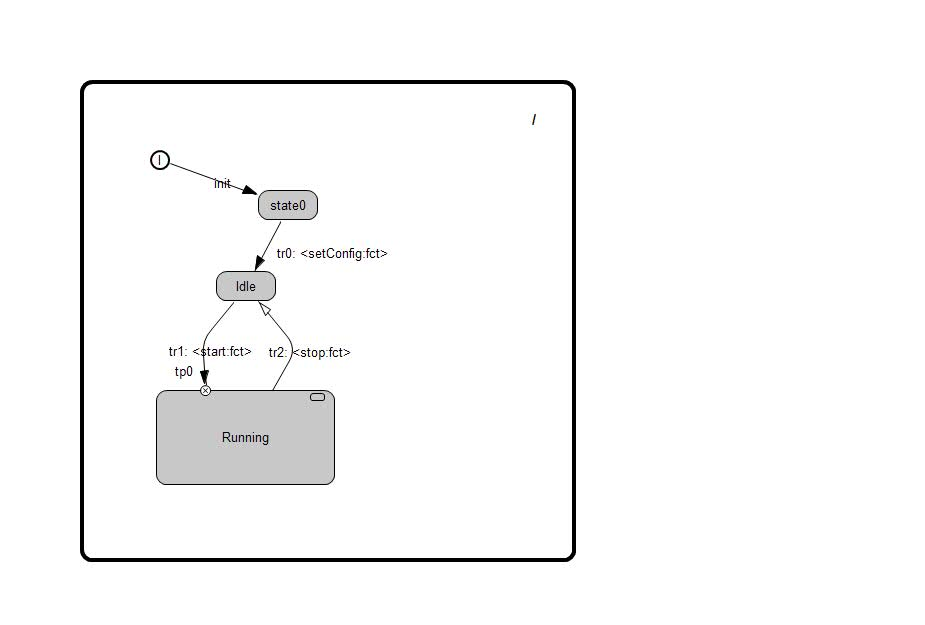
\includegraphics[width=\textwidth]{images/300-Pump_behavior.jpg}
		
		\subsubsection{SubSystemClass}
			\hypertarget{ref:SubSystemClass}{}
			
			The SubSystem is main Actor of an executable part of the system. It instantiates the Actor instance tree instance of the application ...
				
				Actor instance tree example:
			
			
			\vspace{\baselineskip}
			\begingroup
			%\setlength{\tabcolsep}{10pt} % Default value: 6pt
			\renewcommand{\arraystretch}{1.8} % Default value: 1
			\parbox{\textwidth}{
			\begin{longtable}{l l p{.7\textwidth}}
				\multicolumn{2}{l}{\textbf{\large Features}} & \\
				\hline
			\multirow{5}{*}{Contains:} & \tabitem \hyperlink{ref:ActorRef}{ActorRef}  & An ActorRef ...description\\
			& \tabitem \hyperlink{ref:RelayPort}{RelayPort}  & RelayPort description \\
			& \tabitem \hyperlink{ref:SPP}{SPP}  & An SPP ... description \\
			& \tabitem \hyperlink{ref:Binding}{Binding}  & A Binding connects two Ports with each otherdescription \\
			& \tabitem \hyperlink{ref:LayerConnection}{LayerConnection}  & A LayerConnection ... description  \\
			\hline
			\end{longtable}	
			}
			\endgroup
			\vspace{\baselineskip}
			
			\vspace{\baselineskip}
			\begingroup
			%\setlength{\tabcolsep}{10pt} % Default value: 6pt
			\renewcommand{\arraystretch}{1.8} % Default value: 1
			\parbox{\textwidth}{
			\begin{longtable}{l l p{.6\textwidth}}
				\multicolumn{2}{l}{\textbf{\large Related Features}} & \\
				\hline
			Typecasts: & \tabitem \hyperlink{ref:SubSystemRef}{SubSystemRef}  & \\
			\hline
			Is contained in: & \tabitem \hyperlink{ref:LogicalModel}{LogicalModel}  & The LogicalModel describes the logical structure and behavior of a ROOM application. The LogicalModel an its elements can be mapped on any PhysicalModel and its elements...\\
			\hline
			\end{longtable}	
			}
			\endgroup
			\vspace{\baselineskip}
			
			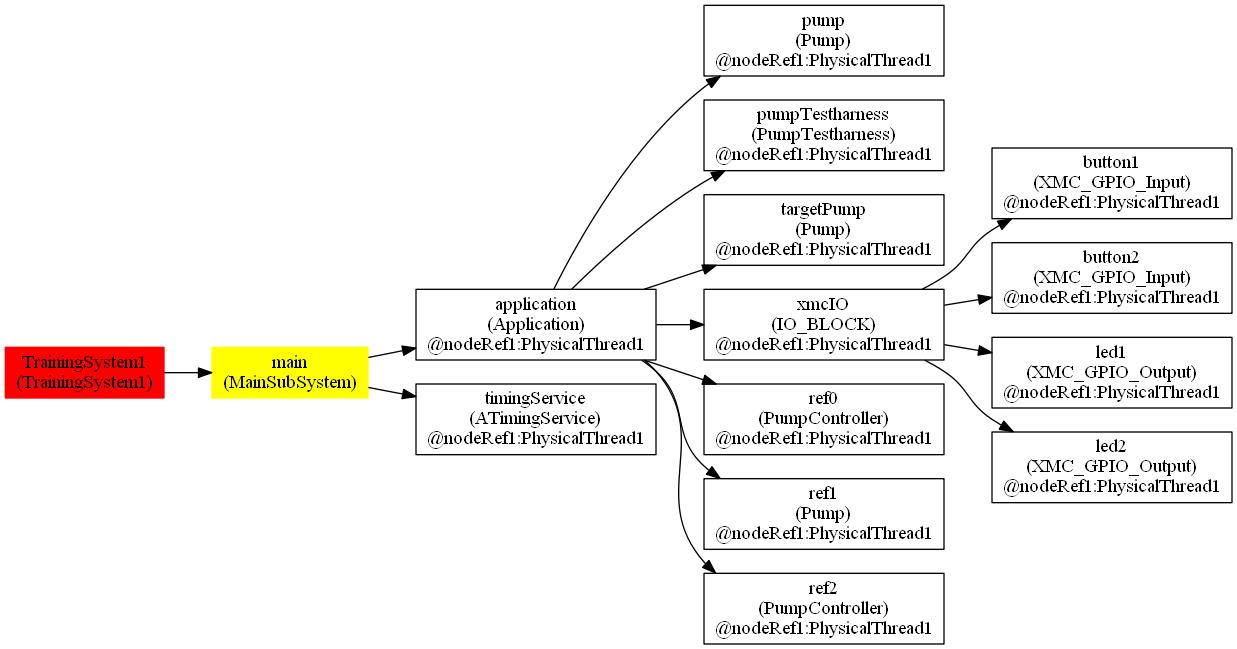
\includegraphics[width=\textwidth]{images/300-TrainingSystem1_instanceTree.jpg}
			
		\subsection{PhysicalModel}
		The PhysicalModel describes the topology of the targets a distributed system can be deployed (mapped) on.
	
		
		\subsection{MappingModel}
		The MappingModel describes the mapping of elements of the LogicalModel to elements of the PhysicalModel. It enables the complete decoupling of the LogicalModel and the PhysicalModel, thus providing a maximum flexibility and reuse for the models.
	
		
		\subsection{ConfigModel}
		The ConfigModel describes the Attribute configuration of ActorInstances and PortInstances. 
	
		
\section{ModelEditors}
	
		\subsection{TextualROOMEditor}
		Textual model editor
	
		
		\subsection{GraphicalStructureEditor}
		The Structure Editor allows to edit the Actor Structure in a convenient way. It is possible to create and arrange actor references and ports and to create bindings and layer connections.
	
		
		
		\subsubsection{ActorRefPropertyDialog}
			\hypertarget{ref:ActorRefPropertyDialog}{}
			
			A Dialog to edit structural reference of an ActorRef.
			
			
			\vspace{\baselineskip}
			\begingroup
			%\setlength{\tabcolsep}{10pt} % Default value: 6pt
			\renewcommand{\arraystretch}{1.8} % Default value: 1
			\parbox{\textwidth}{
			\begin{longtable}{l l p{.7\textwidth}}
				\multicolumn{2}{l}{\textbf{\large Features}} & \\
				\hline
			Edits: & \tabitem \hyperlink{ref:ActorRef}{ActorRef}  & An ActorRef ...description\\
			\hline
			\end{longtable}	
			}
			\endgroup
			\vspace{\baselineskip}
			
			\vspace{\baselineskip}
			\begingroup
			%\setlength{\tabcolsep}{10pt} % Default value: 6pt
			\renewcommand{\arraystretch}{1.8} % Default value: 1
			\parbox{\textwidth}{
			\begin{longtable}{l l p{.6\textwidth}}
				\multicolumn{2}{l}{\textbf{\large Related Features}} & \\
				\hline
			Is contained in: & \tabitem \hyperlink{ref:GraphicalStructureEditor}{GraphicalStructureEditor}  & The Structure Editor allows to edit the Actor Structure in a convenient way. It is possible to create and arrange actor references and ports and to create bindings and layer connections.\\
			\hline
			\end{longtable}	
			}
			\endgroup
			\vspace{\baselineskip}
			
			
		
		\subsubsection{PortPropertyDialog}
			\hypertarget{ref:PortPropertyDialog}{}
			
			
			
			\vspace{\baselineskip}
			\begingroup
			%\setlength{\tabcolsep}{10pt} % Default value: 6pt
			\renewcommand{\arraystretch}{1.8} % Default value: 1
			\parbox{\textwidth}{
			\begin{longtable}{l l p{.7\textwidth}}
				\multicolumn{2}{l}{\textbf{\large Features}} & \\
				\hline
			Edits: & \tabitem \hyperlink{ref:Port}{Port}  & A Port is an instance of a ProtocolClass and the only interface for an ActorClass. It provides strong decoupling of ActorClasses from each other, thus enabling easy testability, reusability and deployment of Actors to different threads or nodes.description \\
			\hline
			\end{longtable}	
			}
			\endgroup
			\vspace{\baselineskip}
			
			\vspace{\baselineskip}
			\begingroup
			%\setlength{\tabcolsep}{10pt} % Default value: 6pt
			\renewcommand{\arraystretch}{1.8} % Default value: 1
			\parbox{\textwidth}{
			\begin{longtable}{l l p{.6\textwidth}}
				\multicolumn{2}{l}{\textbf{\large Related Features}} & \\
				\hline
			Is contained in: & \tabitem \hyperlink{ref:GraphicalStructureEditor}{GraphicalStructureEditor}  & The Structure Editor allows to edit the Actor Structure in a convenient way. It is possible to create and arrange actor references and ports and to create bindings and layer connections.\\
			\hline
			\end{longtable}	
			}
			\endgroup
			\vspace{\baselineskip}
			
			
		
		\subsubsection{SPPPropertyDialog}
			\hypertarget{ref:SPPPropertyDialog}{}
			
			
			
			\vspace{\baselineskip}
			\begingroup
			%\setlength{\tabcolsep}{10pt} % Default value: 6pt
			\renewcommand{\arraystretch}{1.8} % Default value: 1
			\parbox{\textwidth}{
			\begin{longtable}{l l p{.7\textwidth}}
				\multicolumn{2}{l}{\textbf{\large Features}} & \\
				\hline
			Edits: & \tabitem \hyperlink{ref:SPP}{SPP}  & An SPP ... description\\
			\hline
			\end{longtable}	
			}
			\endgroup
			\vspace{\baselineskip}
			
			\vspace{\baselineskip}
			\begingroup
			%\setlength{\tabcolsep}{10pt} % Default value: 6pt
			\renewcommand{\arraystretch}{1.8} % Default value: 1
			\parbox{\textwidth}{
			\begin{longtable}{l l p{.6\textwidth}}
				\multicolumn{2}{l}{\textbf{\large Related Features}} & \\
				\hline
			Is contained in: & \tabitem \hyperlink{ref:GraphicalStructureEditor}{GraphicalStructureEditor}  & The Structure Editor allows to edit the Actor Structure in a convenient way. It is possible to create and arrange actor references and ports and to create bindings and layer connections.\\
			\hline
			\end{longtable}	
			}
			\endgroup
			\vspace{\baselineskip}
			
			
		
		\subsubsection{StructureEditiorPalette}
			\hypertarget{ref:StructureEditiorPalette}{}
			
			creates all Kinds of ...  picture with explanation
			
			
			
			\vspace{\baselineskip}
			\begingroup
			%\setlength{\tabcolsep}{10pt} % Default value: 6pt
			\renewcommand{\arraystretch}{1.8} % Default value: 1
			\parbox{\textwidth}{
			\begin{longtable}{l l p{.6\textwidth}}
				\multicolumn{2}{l}{\textbf{\large Related Features}} & \\
				\hline
			Is contained in: & \tabitem \hyperlink{ref:GraphicalStructureEditor}{GraphicalStructureEditor}  & The Structure Editor allows to edit the Actor Structure in a convenient way. It is possible to create and arrange actor references and ports and to create bindings and layer connections.\\
			\hline
			\end{longtable}	
			}
			\endgroup
			\vspace{\baselineskip}
			
			
		\subsection{GraphicalBehaviorEditor}
		ModelEditor
	
		
\section{CodeGenerators}
	
		\subsection{CCodeGenerator}
	
		
		\subsection{JavaCodeGenerator}
	
		

